% !TEX program = xelatex
\documentclass[12pt,a4paper]{article}

\usepackage{fontspec}
\usepackage{polyglossia}
\setmainlanguage{greek}
\setotherlanguage{english}
\setmainfont[Script=Greek]{DejaVu Serif}
\setsansfont[Script=Greek]{DejaVu Sans}
\setmonofont[Script=Greek]{DejaVu Sans Mono}
\newfontfamily\greekfonttt[Script=Greek]{DejaVu Sans Mono}

\usepackage[a4paper, margin=2.35cm]{geometry}
\usepackage{amsmath, amssymb}
\usepackage{booktabs}
\usepackage{array}
\usepackage{graphicx}
\usepackage{float}
\usepackage{caption}
\usepackage{subcaption}
\usepackage[hidelinks]{hyperref}
\usepackage{enumitem}
\usepackage{parskip}
\usepackage{xcolor}
\usepackage{fancyhdr}

\pagestyle{fancy}
\fancyhf{}
\lhead{Ανάλυση Δεδομένων 2025--26}
\rhead{5η Εργασία -- ΑΕΜ 6931}
\cfoot{\thepage}
\setlength{\headheight}{14.5pt}

\newcommand{\code}[1]{\texttt{\textenglish{#1}}}

\title{
    \textbf{Ανάλυση Δεδομένων 2025--26}\\[0.25cm]
    \Large 5η Εργασία: Νευρωνικά Δίκτυα και CNN στο MNIST\\[0.15cm]
    \large Ταξινόμηση εικόνων χειρόγραφων ψηφίων
}
\author{
    Ρακοβαλής Παύλος\\
    ΑΕΜ: 6931
}
\date{Ιούνιος 2026}

\begin{document}
\sloppy

\maketitle
\thispagestyle{fancy}

\begin{abstract}
Στην εργασία εκπαιδεύονται δύο νευρωνικά δίκτυα για αυτόματη ταξινόμηση
χειρόγραφων ψηφίων του MNIST. Πρώτα χρησιμοποιείται ένα απλό πλήρως συνδεδεμένο
νευρωνικό δίκτυο πάνω σε flattened εικόνες και στη συνέχεια ένα συνελικτικό
νευρωνικό δίκτυο, το οποίο αξιοποιεί τη χωρική δομή των εικόνων. Τα δεδομένα
δειγματοληπτούνται με seed τον ΑΕΜ 6931: 90\% του αρχικού train set και 80\%
του αρχικού test set. Το CNN πέτυχε υψηλότερη ακρίβεια στο test set
(\(98.99\%\)) από το απλό NN (\(97.56\%\)), ενώ είχε και λιγότερες παραμέτρους.
\end{abstract}

\tableofcontents
\newpage

%=============================================================================
\section{Δεδομένα και προεπεξεργασία}
%=============================================================================

Το σύνολο MNIST αποτελείται από grayscale εικόνες χειρόγραφων ψηφίων, με
διαστάσεις \(28 \times 28\) pixels. Κάθε εικόνα ανήκει σε μία από τις 10
κλάσεις, δηλαδή στα ψηφία 0 έως 9.

Σύμφωνα με την εκφώνηση, έγινε τυχαία δειγματοληψία με seed τον ΑΕΜ:

\[
    \text{\code{random\_state}} = 6931.
\]

Από τα αρχικά δεδομένα επιλέχθηκαν:

\begin{center}
\begin{tabular}{lrr}
\toprule
\textbf{Σύνολο} & \textbf{Αρχικό πλήθος} & \textbf{Πλήθος μετά τη δειγματοληψία} \\
\midrule
Train set & 60000 & 54000 \\
Test set  & 10000 & 8000 \\
\bottomrule
\end{tabular}
\end{center}

\subsection{Shape των δεδομένων και πλήθος κλάσεων}

Μετά τη δειγματοληψία, τα δεδομένα έχουν τα εξής σχήματα:

\begin{center}
\begin{tabular}{ll}
\toprule
\textbf{Πίνακας} & \textbf{Shape} \\
\midrule
\code{x\_train} ως εικόνες & \((54000, 28, 28)\) \\
\code{y\_train} & \((54000,)\) \\
\code{x\_test} ως εικόνες & \((8000, 28, 28)\) \\
\code{y\_test} & \((8000,)\) \\
\code{x\_train} flattened & \((54000, 784)\) \\
\code{x\_test} flattened & \((8000, 784)\) \\
\code{x\_train} για CNN & \((54000, 28, 28, 1)\) \\
\code{x\_test} για CNN & \((8000, 28, 28, 1)\) \\
\bottomrule
\end{tabular}
\end{center}

Το πλήθος των κλάσεων είναι:
\[
    K = 10.
\]

\subsection{Ισορροπία κλάσεων}

\begin{table}[H]
\centering
\caption{Πλήθος δειγμάτων ανά ψηφίο μετά τη δειγματοληψία.}
\begin{tabular}{crr}
\toprule
\textbf{Ψηφίο} & \textbf{Train sample} & \textbf{Test sample} \\
\midrule
0 & 5329 & 792 \\
1 & 6060 & 905 \\
2 & 5350 & 810 \\
3 & 5522 & 820 \\
4 & 5279 & 791 \\
5 & 4887 & 707 \\
6 & 5347 & 775 \\
7 & 5614 & 827 \\
8 & 5232 & 774 \\
9 & 5380 & 799 \\
\bottomrule
\end{tabular}
\end{table}

Οι κλάσεις είναι αρκετά ισορροπημένες. Υπάρχουν μικρές διαφορές, με το ψηφίο
1 να εμφανίζεται συχνότερα και το ψηφίο 5 λιγότερο συχνά, όμως καμία κλάση δεν
λείπει και οι αναλογίες παραμένουν κοντά στο 10\%.

\begin{figure}[H]
\centering
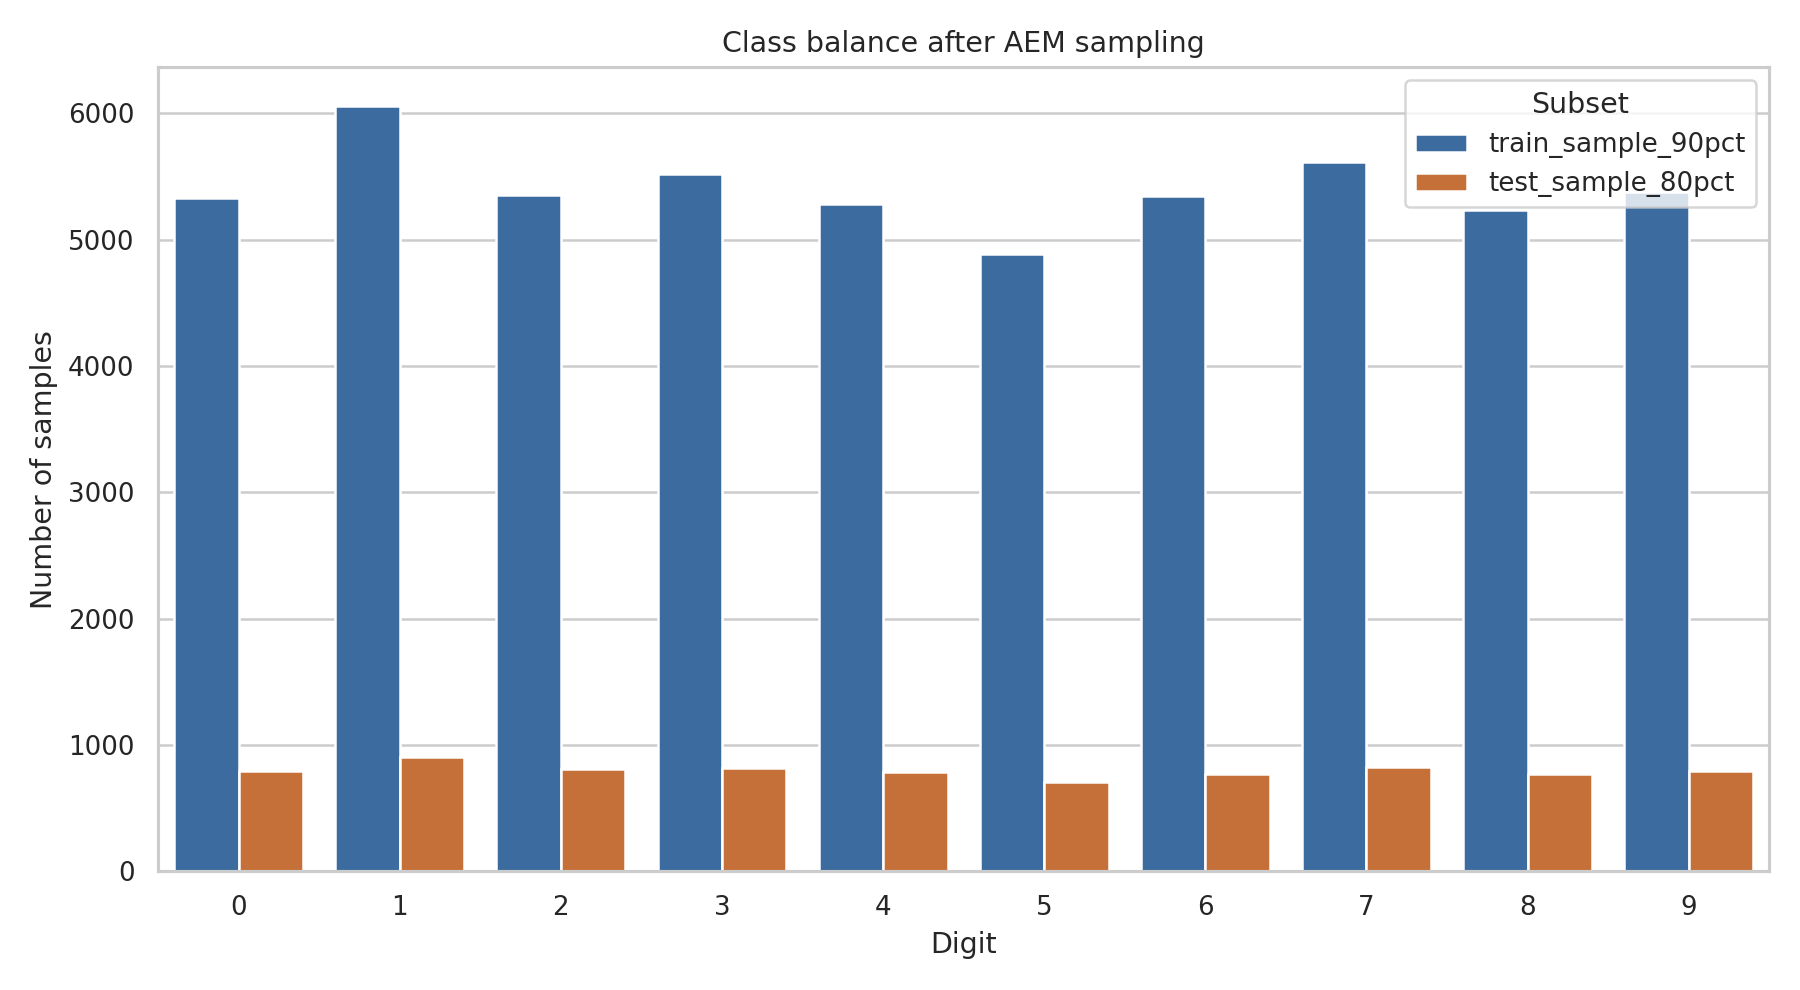
\includegraphics[width=0.82\textwidth]{outputs/class_balance.png}
\caption{Κατανομή των κλάσεων στα δειγματοληπτημένα train και test sets.}
\end{figure}

\begin{figure}[H]
\centering
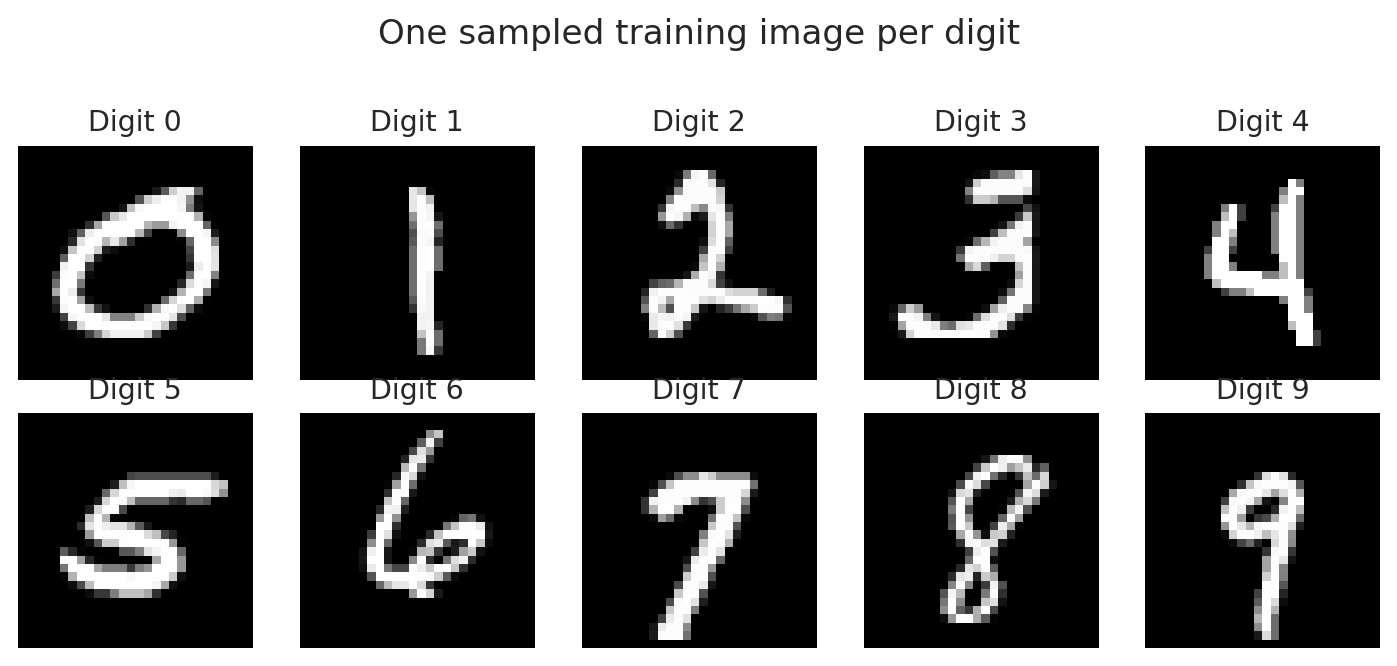
\includegraphics[width=0.78\textwidth]{outputs/sample_digits.png}
\caption{Ενδεικτική εικόνα από κάθε ψηφίο στο training set.}
\end{figure}

\subsection{Κανονικοποίηση}

Οι αρχικές τιμές των pixels βρίσκονται στο διάστημα \([0,255]\). Για την
εκπαίδευση των νευρωνικών δικτύων μετατράπηκαν στο διάστημα \([0,1]\):

\[
    x_{\text{norm}} = \frac{x}{255}.
\]

Η κανονικοποίηση βοηθά στη σύγκλιση, επειδή όλες οι είσοδοι αποκτούν κοινή
κλίμακα. Έτσι οι ενημερώσεις των βαρών μέσω backpropagation γίνονται πιο
σταθερές, αποφεύγονται πολύ μεγάλες ενεργοποιήσεις και ο optimizer μπορεί να
κινηθεί πιο ομαλά προς ένα καλό ελάχιστο της συνάρτησης απώλειας.

\subsection{Flattening}

Για το απλό πλήρως συνδεδεμένο νευρωνικό δίκτυο, κάθε εικόνα
\(28 \times 28\) μετατράπηκε σε διάνυσμα 784 στοιχείων:

\[
    28 \cdot 28 = 784.
\]

Το flattening είναι απαραίτητο για Dense επίπεδα, επειδή αυτά δέχονται ως
είσοδο μονοδιάστατα διανύσματα χαρακτηριστικών. Το μειονέκτημα είναι ότι
χάνεται η άμεση χωρική πληροφορία της εικόνας, δηλαδή το ποια pixels είναι
γειτονικά μεταξύ τους. Αυτό είναι ένας από τους λόγους που τα CNN είναι πιο
κατάλληλα για εικόνες.

%=============================================================================
\section{Ενότητα Α: Απλό Νευρωνικό Δίκτυο}
%=============================================================================

\subsection{Αρχιτεκτονική}

Το απλό μοντέλο είναι \code{Sequential} και αποτελείται από Dense επίπεδα:

\begin{center}
\begin{tabular}{llr}
\toprule
\textbf{Επίπεδο} & \textbf{Ενεργοποίηση} & \textbf{Νευρώνες} \\
\midrule
Input/Dense & ReLU & 784 \\
Hidden 1 & ReLU & 256 \\
Hidden 2 & ReLU & 128 \\
Output & Softmax & 10 \\
\bottomrule
\end{tabular}
\end{center}

Η συνάρτηση ReLU χρησιμοποιείται στα ενδιάμεσα επίπεδα, επειδή είναι απλή,
υπολογιστικά αποδοτική και βοηθά στην εκπαίδευση βαθύτερων δικτύων περιορίζοντας
το πρόβλημα των πολύ μικρών gradients. Στο output χρησιμοποιείται Softmax, ώστε
το μοντέλο να δίνει πιθανότητες για τις 10 κλάσεις.

\subsection{Optimizer και loss function}

Ως optimizer χρησιμοποιήθηκε ο \code{Adam}. Ο Adam προσαρμόζει το learning rate
ανά παράμετρο και συνήθως συγκλίνει γρήγορα σε προβλήματα ταξινόμησης εικόνων.

Ως συνάρτηση απώλειας χρησιμοποιήθηκε η \textenglish{sparse categorical crossentropy}.
Είναι κατάλληλη επειδή έχουμε πολυταξική ταξινόμηση 10 αμοιβαία αποκλειόμενων
κλάσεων και τα labels δίνονται ως ακέραιοι αριθμοί 0 έως 9, όχι ως one-hot
vectors.

Η εκπαίδευση έγινε για 30 epochs με validation split 10\%. Άρα από τα 54000
training δείγματα, περίπου 48600 χρησιμοποιούνται για εκπαίδευση και 5400 για
validation σε κάθε epoch.

\subsection{Αποτελέσματα εκπαίδευσης}

\begin{figure}[H]
\centering
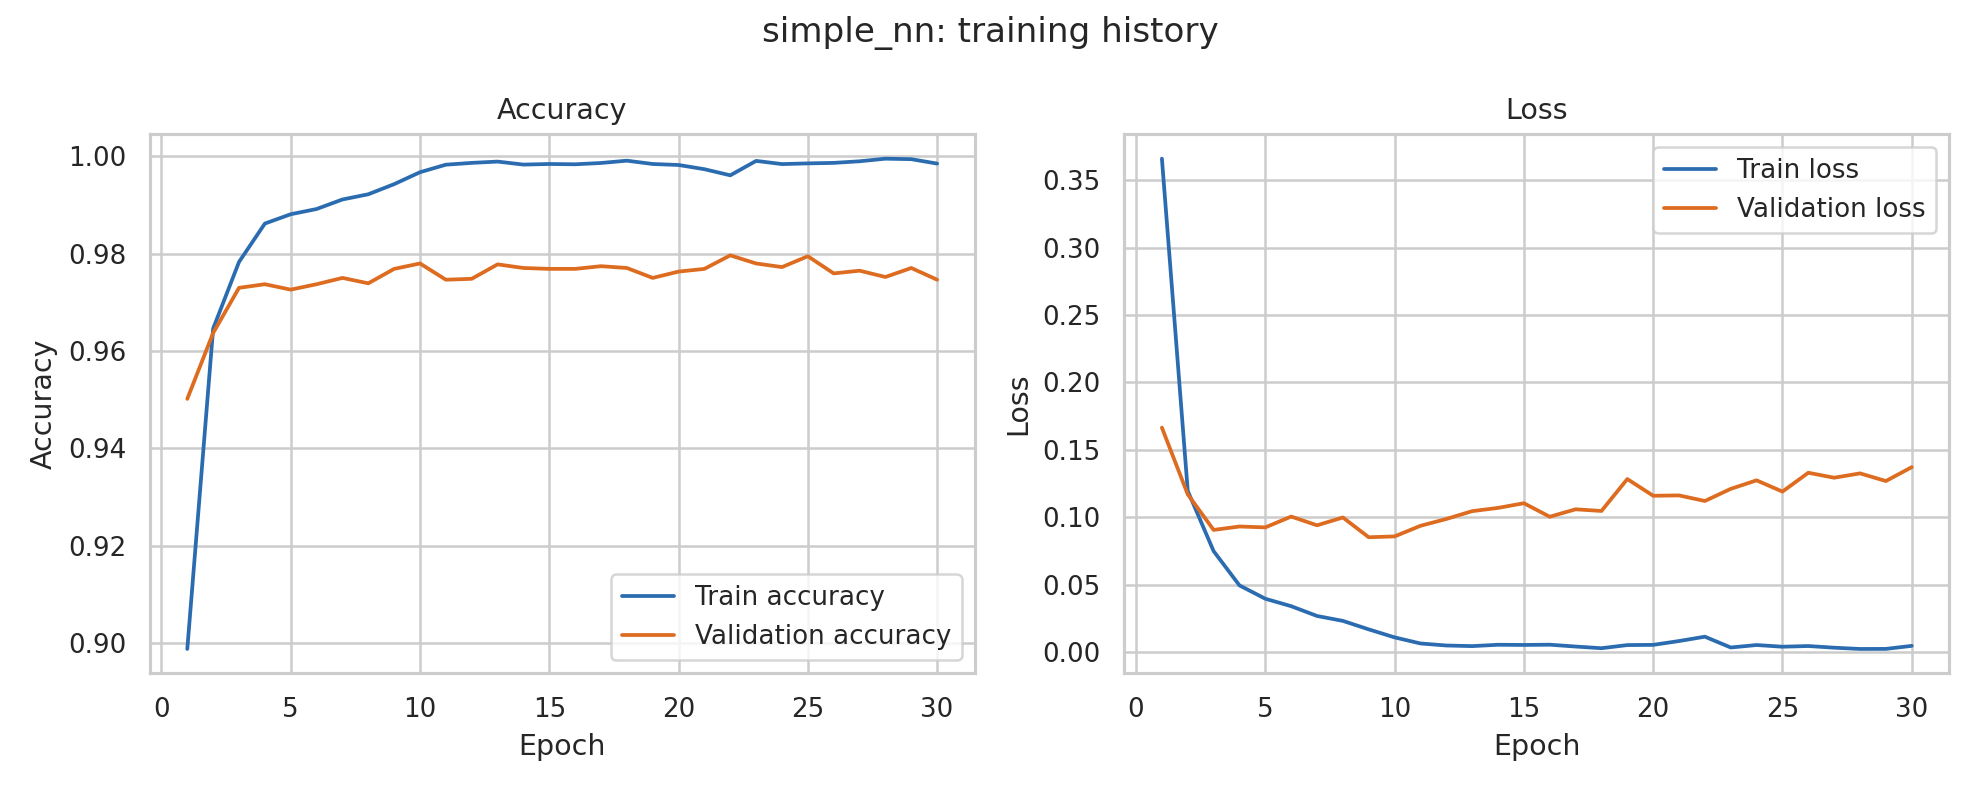
\includegraphics[width=\textwidth]{outputs/simple_nn_history.png}
\caption{Καμπύλες accuracy και loss για το απλό νευρωνικό δίκτυο.}
\end{figure}

Στο τέλος των 30 epochs προέκυψαν:

\begin{center}
\begin{tabular}{lr}
\toprule
\textbf{Μέγεθος} & \textbf{Τιμή} \\
\midrule
Train accuracy & 0.9985 \\
Validation accuracy & 0.9746 \\
Train loss & 0.0046 \\
Validation loss & 0.1372 \\
Test accuracy & 0.9756 \\
Test loss & 0.1315 \\
Παράμετροι & 850586 \\
\bottomrule
\end{tabular}
\end{center}

\subsection{Πίνακας σύγχυσης}

\begin{figure}[H]
\centering
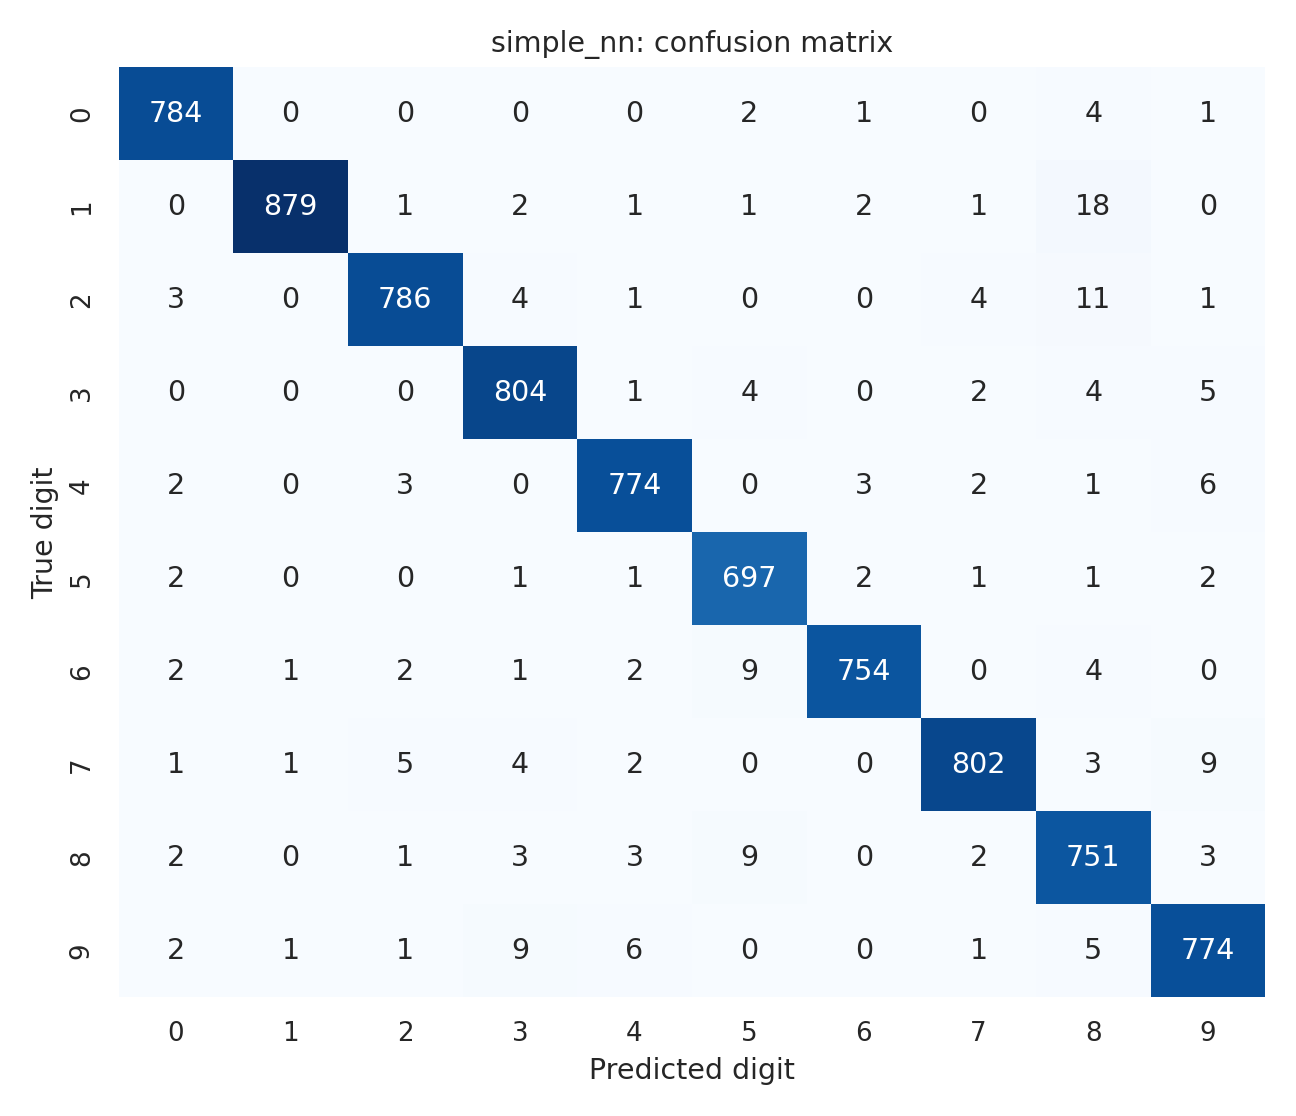
\includegraphics[width=0.72\textwidth]{outputs/simple_nn_confusion_matrix.png}
\caption{Πίνακας σύγχυσης για το απλό νευρωνικό δίκτυο στο test set.}
\end{figure}

Τα συχνότερα λάθη του απλού NN ήταν:

\begin{center}
\begin{tabular}{lrr}
\toprule
\textbf{Πραγματικό ψηφίο} & \textbf{Πρόβλεψη} & \textbf{Πλήθος} \\
\midrule
1 & 8 & 18 \\
2 & 8 & 11 \\
6 & 5 & 9 \\
7 & 9 & 9 \\
8 & 5 & 9 \\
9 & 3 & 9 \\
\bottomrule
\end{tabular}
\end{center}

Τα λάθη αυτά σχετίζονται κυρίως με μορφολογικές ομοιότητες σε χειρόγραφες
μορφές. Για παράδειγμα, το 7 μπορεί να μοιάζει με 9 όταν έχει έντονη καμπύλη,
το 9 μπορεί να μοιάζει με 3 όταν η κάθετη ουρά είναι αχνή, ενώ το 8 μπορεί να
μπερδευτεί με 5 σε εικόνες όπου ο κάτω λοβός είναι πιο έντονος από τον πάνω.
Το απλό NN βλέπει την εικόνα ως απλό διάνυσμα 784 αριθμών και δεν αξιοποιεί
ρητά τις τοπικές σχέσεις ανάμεσα σε γειτονικά pixels, άρα είναι πιο ευάλωτο σε
τέτοιες μικρές μετατοπίσεις και παραμορφώσεις.

\subsection{Overfitting}

Παρατηρείται ένδειξη overfitting. Το train accuracy φτάνει πολύ κοντά στο 1,
ενώ το validation accuracy σταθεροποιείται περίπου στο 0.975. Παράλληλα, το
train loss γίνεται σχεδόν μηδενικό, ενώ το validation loss αυξάνεται στα
τελευταία epochs. Αυτό σημαίνει ότι το μοντέλο μαθαίνει πολύ καλά τα training
δεδομένα, αλλά η επιπλέον εκπαίδευση δεν βελτιώνει αντίστοιχα τη γενίκευση.

%=============================================================================
\section{Ενότητα Β: Συνελικτικό Νευρωνικό Δίκτυο}
%=============================================================================

\subsection{Αρχιτεκτονική CNN}

Το CNN δέχεται ως είσοδο τις εικόνες στη μορφή \((28,28,1)\), ώστε να
διατηρείται η χωρική δομή και το κανάλι grayscale.

\begin{center}
\begin{tabular}{llr}
\toprule
\textbf{Επίπεδο} & \textbf{Ρύθμιση} & \textbf{Παράμετροι} \\
\midrule
Conv2D & 32 φίλτρα \(3 \times 3\), ReLU & 320 \\
MaxPooling2D & Παράθυρο \(2 \times 2\) & 0 \\
Conv2D & 64 φίλτρα \(3 \times 3\), ReLU & 18496 \\
Flatten & -- & 0 \\
Dense & 64 νευρώνες, ReLU & 495680 \\
Output Dense & 10 νευρώνες, Softmax & 650 \\
\midrule
\textbf{Σύνολο} & & \textbf{515146} \\
\bottomrule
\end{tabular}
\end{center}

Το CNN εκπαιδεύτηκε επίσης με Adam, \textenglish{sparse categorical crossentropy},
30 epochs και validation split 10\%.

\subsection{Αποτελέσματα εκπαίδευσης}

\begin{figure}[H]
\centering
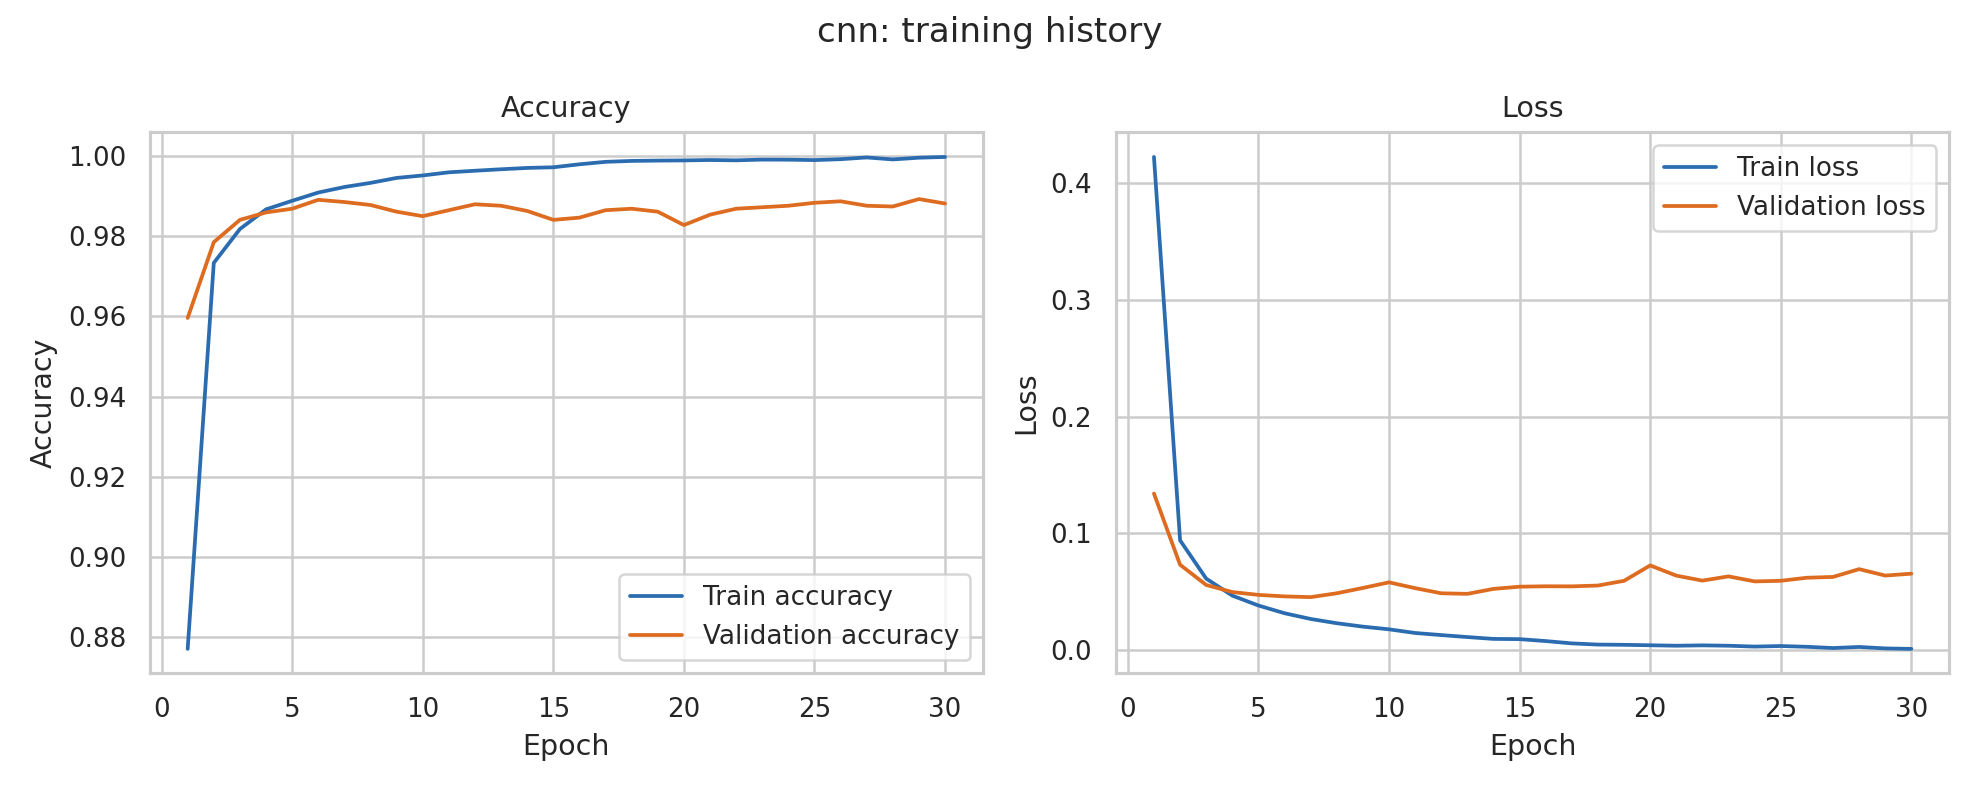
\includegraphics[width=\textwidth]{outputs/cnn_history.png}
\caption{Καμπύλες accuracy και loss για το CNN.}
\end{figure}

Στο τέλος των 30 epochs προέκυψαν:

\begin{center}
\begin{tabular}{lr}
\toprule
\textbf{Μέγεθος} & \textbf{Τιμή} \\
\midrule
Train accuracy & 0.9998 \\
Validation accuracy & 0.9881 \\
Train loss & 0.0010 \\
Validation loss & 0.0654 \\
Test accuracy & 0.9899 \\
Test loss & 0.0469 \\
Παράμετροι & 515146 \\
\bottomrule
\end{tabular}
\end{center}

\subsection{Πίνακας σύγχυσης}

\begin{figure}[H]
\centering
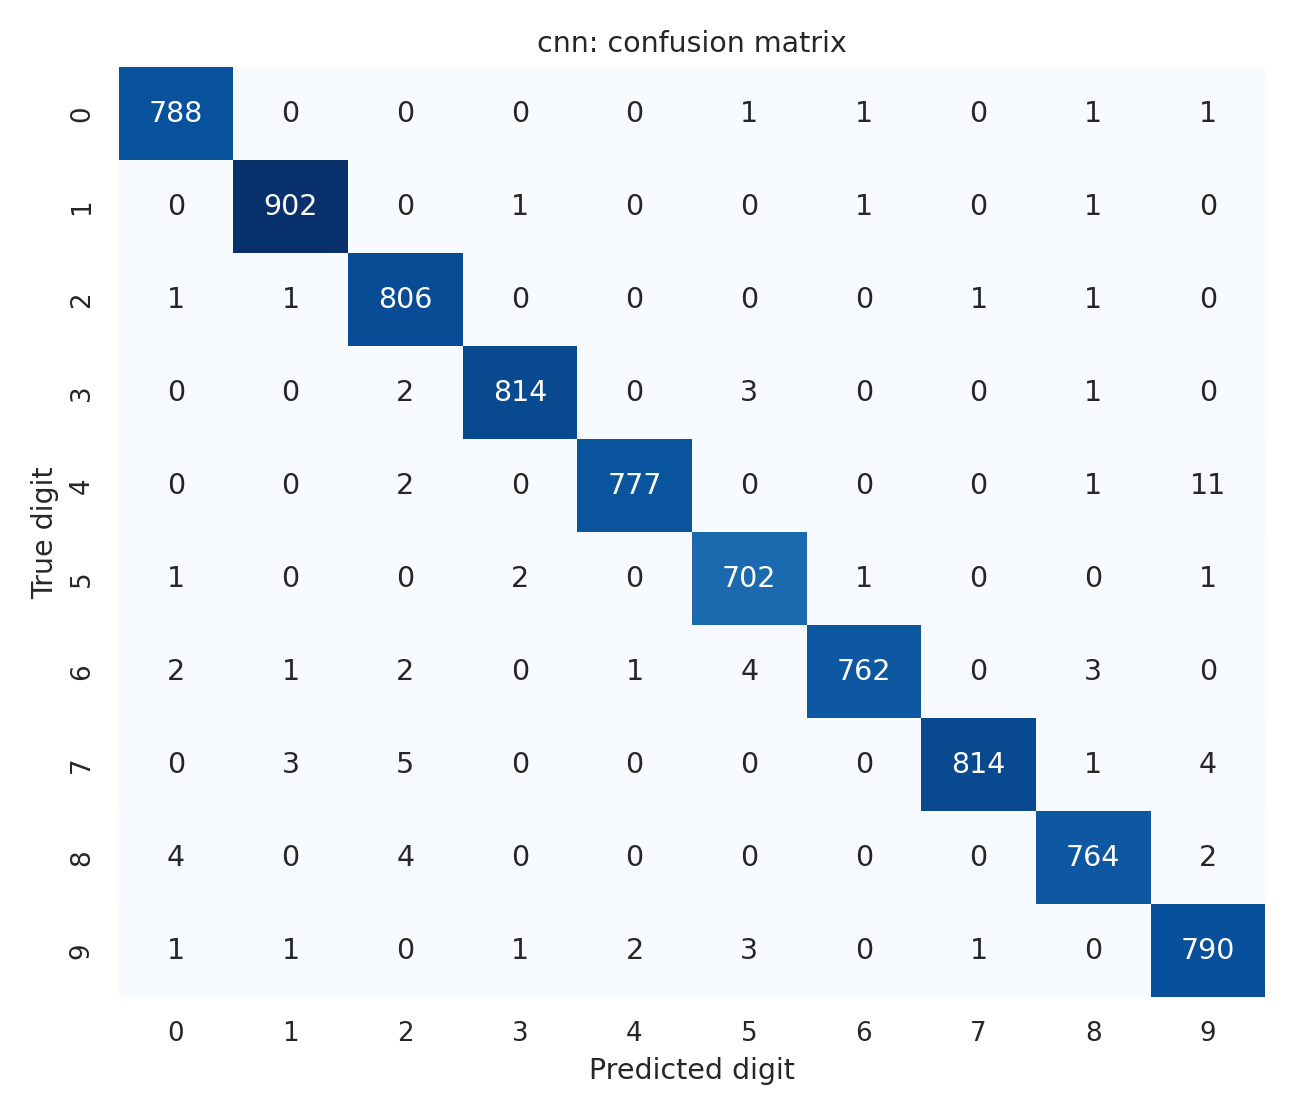
\includegraphics[width=0.72\textwidth]{outputs/cnn_confusion_matrix.png}
\caption{Πίνακας σύγχυσης για το CNN στο test set.}
\end{figure}

Τα συχνότερα λάθη του CNN ήταν:

\begin{center}
\begin{tabular}{lrr}
\toprule
\textbf{Πραγματικό ψηφίο} & \textbf{Πρόβλεψη} & \textbf{Πλήθος} \\
\midrule
4 & 9 & 11 \\
7 & 2 & 5 \\
7 & 9 & 4 \\
6 & 5 & 4 \\
8 & 2 & 4 \\
8 & 0 & 4 \\
\bottomrule
\end{tabular}
\end{center}

Το συχνότερο μπέρδεμα είναι το \(4 \rightarrow 9\). Αυτό είναι αναμενόμενο σε
χειρόγραφα ψηφία, επειδή κάποια 4 γράφονται με κλειστό πάνω τμήμα και μπορούν
να θυμίσουν 9. Επίσης, το 7 μπορεί να μπερδευτεί με 2 λόγω κοινής λοξής
γραμμής και άνω οριζόντιας γραμμής, ενώ τα 8 και 0 έχουν κοινή κλειστή,
κυκλική μορφή.

%=============================================================================
\section{Σύγκριση μοντέλων}
%=============================================================================

\begin{table}[H]
\centering
\caption{Σύγκριση απλού NN και CNN.}
\begin{tabular}{lrrrr}
\toprule
\textbf{Μοντέλο} & \textbf{Παράμετροι} & \textbf{Val. accuracy} & \textbf{Test accuracy} & \textbf{Test loss} \\
\midrule
Simple NN & 850586 & 0.9746 & 0.9756 & 0.1315 \\
CNN & 515146 & 0.9881 & 0.9899 & 0.0469 \\
\bottomrule
\end{tabular}
\end{table}

Το CNN έχει καλύτερη απόδοση στο test set:

\[
    0.9899 - 0.9756 = 0.0143.
\]

Δηλαδή η ακρίβεια αυξάνεται περίπου κατά 1.43 ποσοστιαίες μονάδες. Επιπλέον,
το CNN έχει λιγότερες παραμέτρους από το απλό NN, παρότι πετυχαίνει καλύτερη
ακρίβεια.

Η διαφορά εξηγείται από τον τρόπο με τον οποίο τα CNN επεξεργάζονται εικόνες.
Τα συνελικτικά φίλτρα μαθαίνουν τοπικά μοτίβα, όπως ακμές, καμπύλες, γωνίες και
μικρά τμήματα ψηφίων. Τα ίδια φίλτρα εφαρμόζονται σε διαφορετικές θέσεις της
εικόνας, άρα το μοντέλο μπορεί να αναγνωρίζει ένα μοτίβο ανεξάρτητα από το αν
εμφανίζεται λίγο πιο πάνω, κάτω, αριστερά ή δεξιά. Το MaxPooling μειώνει τη
διάσταση και κάνει την αναπαράσταση πιο ανθεκτική σε μικρές μετατοπίσεις.

Αντίθετα, το απλό NN αντιμετωπίζει κάθε pixel ως ξεχωριστό χαρακτηριστικό.
Έτσι μπορεί να μάθει χρήσιμα μοτίβα, αλλά δεν έχει ενσωματωμένη γνώση ότι
γειτονικά pixels σχηματίζουν τοπικές δομές. Για αυτό τα CNN θεωρούνται γενικά
καταλληλότερα για εικόνες.

\subsection{Συμπέρασμα}

Και τα δύο μοντέλα ταξινομούν με υψηλή ακρίβεια τα ψηφία του MNIST. Ωστόσο,
το CNN είναι σαφώς πιο κατάλληλο για το συγκεκριμένο πρόβλημα, επειδή αξιοποιεί
τη χωρική πληροφορία των εικόνων. Στο πείραμα της εργασίας πέτυχε υψηλότερη
test accuracy, χαμηλότερο test loss και μικρότερο πλήθος παραμέτρων από το
απλό πλήρως συνδεδεμένο νευρωνικό δίκτυο.

\end{document}
